\documentclass[runningheads,a4paper]{llncs}

\usepackage[BoldFont,SlantFont,CJKsetspaces,CJKchecksingle]{xeCJK}
\setCJKmainfont[BoldFont=SimHei]{SimSun}
\setCJKmonofont{SimSun}% 设置缺省中文字体

\usepackage{amssymb}
\usepackage{graphicx}
%\usepackage{multirow}
\usepackage{url}
\usepackage{color}
\usepackage{CJKutf8}
\usepackage{url}
\usepackage[ruled]{algorithm2e}
\usepackage{amsmath}
\usepackage{graphicx}
\usepackage{enumerate}

\urldef{\mailthu}\path|{lmy13@}tsinghua.edu.cn|
\urldef{\mailsy}\path|{fantasysy@}sina.com|
\newcommand{\keywords}[1]{\par\addvspace\baselineskip\noindent\keywordname\enspace\ignorespaces#1}
\newcommand{\para}[1]{\vspace{0.1cm}\noindent\textbf{#1}}

\begin{document}
\mainmatter

\title{Building Large-Scale Cross-lingual Knowledge Base from Multi-Encyclopedia}
\titlerunning{Bilingual Knowledge Base}
\author{Mingyang Li$^\dag$ \and Yao Shi$^\dag$ \and Zhigang Wang$^\dag$}
\authorrunning{Mingyang Li et.al}

\institute{$^\dag$Tsinghua National Laboratory for Information Science and Technology,\\
Department of Computer Science and Technology,\\
Tsinghua University, Beijing 100084, China\\
\mailthu\\
\mailsy\\
}

\maketitle

\begin{abstract}
    Abstract Text

\keywords{Knowledge Base, Semantic Web, Linked Data, Ontology, Cross-lingual}
\end{abstract}

\section{Introduction}
With LOD growing recent years, more and more knowledge bases are generated in different languages and in various domains. Several large-scale knowledge bases, such as DBpedia\cite{mendes2012dbpedia}, YAGO\cite{mahdisoltani2014yago3} and Freebase\cite{bollacker2008freebase} are well-known and often used for information extraction \cite{dutta2013integrating}, entity linking\cite{shen2012linden}, recommendation\cite{passant2010dbrec,fernandez2011generic,kaminskas2012knowledge}and so on. These knowledge bases are not only cross-domain but also multilingual, which is benefit for global knowledge sharing. 

Take DBpedia as an example, it extracts structural information from Wikipedia, the largest knowledge sharing resource in the world and have already contained approximately 38.3 million things. Right now DBpedia provides 124 versions of non-English language including German, French and Japanese etc. Moreover, there are instances and 11 classes in Chinese. Obviously, the quality of Chinese information is not enough for further research or application. Neither do the other knowledge bases containing Chinese version. 

To build a cross-lingual knowledge base, some problems are to be addressed: (1) The imbalanced size of different Wikipedia languages leads to less data of various languages. In Wikipedia, the number of articles in English has reached almost 5 millions, while in Chinese there are only 800 thousand. The scarcity of resources makes structuring a large-scale cross-lingual knowledge base within Chinese and English difficult. (2) The number of existed cross-lingual links in Wikipedia is so small that affects the quality of a bilingual knowledge base. Especially there is no obvious links in properties.Statistically, only about XX thousand cross-lingual links are between English and Chinese articles. (3) The large but irrigorous category system in Wikipedia causes incorrect semantic relations in taxonomy. For example,\textcolor{red}{example}

%In Semantic Web, a large-scale multilingual knowledge base can help …

%Thus it’s significative to build a Chinese-English knowledge base and benefit from it. 

Currently, there are several massive knowledge encyclopedias in Chinese, including Hudong and Baidu Baike. To solve the unbalance problem, we utilize such seperated resources to enrich our Chinese information. In this paper, we propose an approach to combine four resources, which are English Wikipedia, Chinese Wikipedia, Hudong Baike and Baidu Baike, into one cross-lingual knowledge base, which contains XXX concepts, XXX instances and XXX properties. To get a more available result, we also make judgement on the relation among concepts and instances. At last, a query interface is provided to access the knowledge base. Specifically, our work makes the following contributions:
\begin{itemize}
  \item We propose a method to build a Chinese-English cross-lingual knowledge base combining four encyclopedias, which are English Wikipedia, Chinese Wikipedia, Baidu and Hudong. The latter three contain large amount of Chinese knowledge, which helps balance and enrich information of two languages.
  %\item We extend the cross-lingual link set by employing a cross-lingual knowledge linking discovery approach for concept and instance, and by analysing templates in Wikipedia for property.
  \item We prune the original taxonomy, which is extracted from encyclopedia category system, to retrieve more precise subClassOf and instanceOf relation in ontology.
  \item A website is developed based on our ontology and also a SPARQL interface is provided for public query operations in our knowledge base.
\end{itemize}

The rest of the paper is organized as follows. Section \ref{sec:pre} introduces the four involved encyclopedias. Besides, definitions are proposed in this section. Section \ref{sec:dp} presents the extraction approach in concept, instance and property level. Section \ref{sec:clkbb} describes the procedure of bulding a knowledge base using extracting result. Section \ref{sec:result} shows the results of established knowledge base. Section \ref{sec:work} induces related work about this paper. Section \ref{sec:con} gives the conclusion.

\section{Preliminary}
\label{sec:pre}
In this section, we firstly introduce the four encyclopedias used to build and enrich our knowledge base. Then we give some related definitions to formalize our procedure.

\subsection{Encyclopedias}
\label{sec:encyclopedias}
\subsubsection{Wikipedia}
Nowadays, Wikipedia is the largest data store of human knowledge. It was launched in 2001 and has hold over 35 million articles in 288 language by 2015. Out of these, English articles contribute most. There are 4.8 million articles in English while only over 800thousand articles in Chinese. It is obvious that the quantity of English articles is far more than Chinese. Such imbalance makes those ontologies based on Wikipedia-only behave badly in cross-lingual aspect. For example, DBpedia has 683 concepts in English while only 11 Chinese concepts, that helps little when other poeple want to do cross-lingual research depending on DBpedia. To avoid the imbalance problem, two other Chinese encyclopedias are utilized to extend Chinese source.

Articles in Wikipedia are manually editted by various authors. Wikipedia provides many templates to guide authors composing their context in a standard way, so do infoboxes. For example, The infobox in film 星际穿越(Interstellar) use the Template \emph{Infobox film}. Infobox template maintains a property set of similar articles and display labels on webpage.

\subsubsection{Other Chinese Encyclopedias}
There are several large-scale monolingual Chinese Encyclopedias currently. Among those, Baidu Baike and Hudong Baike are the most well-known. Hudong Baike was founded in 2005 and contains more than 12 millions articles with about 9 millions experts' contribution util 2015. At the mean time, Baidu Baike maintains more than 11 millions articles. These two resources are similar in article structure, somethimes even in content. 

\subsubsection{Encyclopedia Page}
\label{sec:ep}
All these four encyclopedias have two important elements, articles and category taxonomy. A taxonomy presents the relation between categories. Usually a category has its sub-categories and super-categories. Fig.\ref{fig:hudong-taxonomy} shows a screenshot of Hudong Taxonomy. Besides, an article belongs to one or more categories. An article describes an entity with rich information created and modified by several verified editors. The content and relation of an article provide a lot when building a cross-domain knowledge base. In general, there are five elements can be exploited:
\begin{figure}
    \centering
    \begin{minipage}[t]{0.8\textwidth}
        \centerline{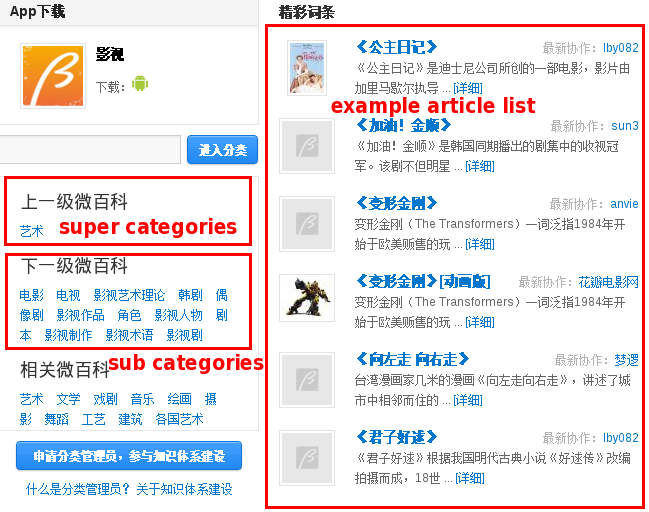
\includegraphics[width=0.8\columnwidth]{fig/hudong-taxonomy2}}
        \label{fig:hudong-taxonomy}
        \caption{Taxonomy in Hudong}
    \end{minipage}%
\end{figure}
\begin{itemize}
  \item Title: A Title is the label of entity, which is unique to an article so that it can be used to distinguish entities.
  \item Abstract: An abstract is a brief summarize of the entity. It's always the first paragraph of an article. Usually it can be taken as an important feature due to the summary content. 
  \item Infobox: Most of articles contain infobox. An infobox maintains structured data which are frequently subject-attribute-value triples formalized as a table. Information in this table includes important properties of an entity.
  \item Links: Links are entries to other articles within the encyclopedia. They lead readers to reference articles. Actually, they represent the relations between the current article and other articles.
  \item Category: The categories that an article belongs to are usually listed at the bottom of article page, shown as tags. An article attaches to one or more categories.
\end{itemize}
Fig. \ref{fig:interstellar} shows a snap of an article in Chinese Wikipedia. 
\begin{figure}[ht]
    \centerline{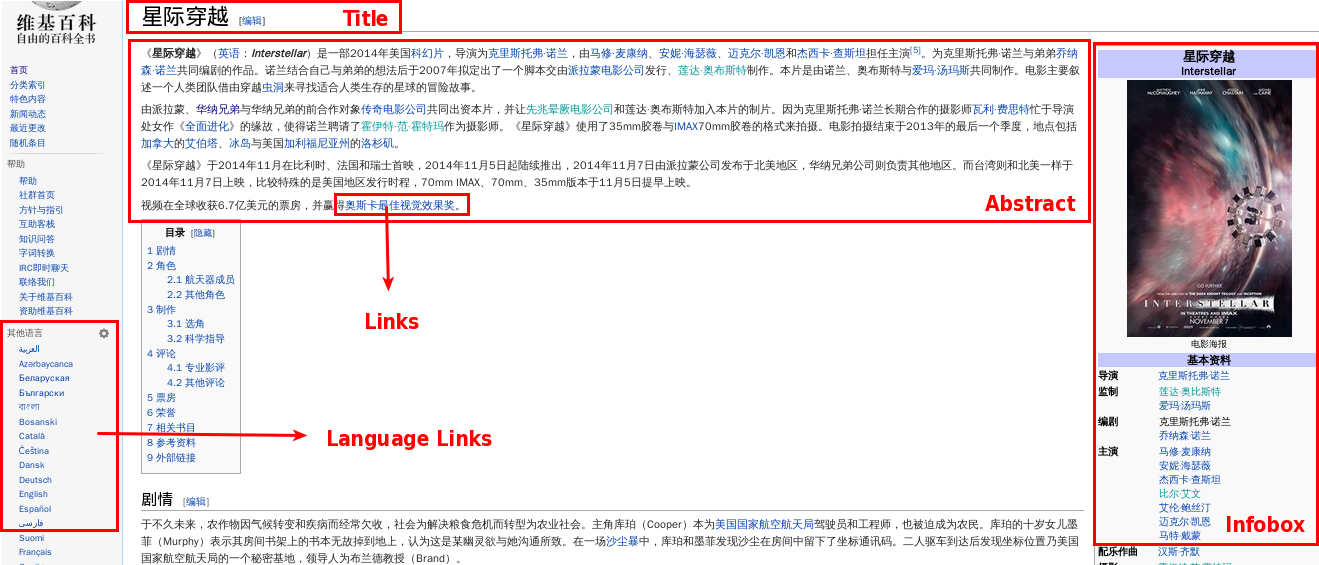
\includegraphics[width=1\columnwidth]{fig/interstellar}}
    \label{fig:interstellar}
    \caption{A snap of Interstellar(Film) article in Chinese Wikipedia}
\end{figure}%

\subsection{Cross-lingual Links}
In order to build a cross-lingual knowledge base, we need the relation between Chinese source and English source, which helps merge different language information into their common entities. In Wikipedia, most articles have language links which guide the reader to the article in specific language under the same entity. Fig. \ref{fig:interstellar}shows language links of \emph{Interstellar} is on the right of Wikipedia page. Taking advantage of human established language links, we can generate an initial cross-lingual ontology based on Chinese and English Wikipedia, similar to DBpedia. Afterwards, to combine Hudong Baike and Baidu Baike, which are lack of cross-lingual information but rich in Chinese data, we employ the approach proposed in \cite{wang2012cross} to discover cross-lingual links between English Wikipedia and Baidu Baike. 

\subsection{Definitions}
\label{sec:definition}
Here we list definitions involved in the later sections:

\textbf{Definition 1:} A Encyclopedia is considered as a collection of articles, category system, which can be defined as: $W = <A,C>$, where A denotes articles, C denotes categories in W.

\textbf{Definition 2:} According to Section \ref{sec:ep}, there are several elements of an article. Therefore, each article $a$ can be defined as follow:
\begin{equation}
    a = <Ti(a),AB(a),Li(a),I(a),C(a)>
\end{equation}
where $Ti(a),AB(a),Li(a),I(a),C(a)$ denotes title, abstract, links, infobox, category tag of article a.

\textbf{Definition 3:} To an article $a$ containing multi-language content in Wikipedia, $L_{e}$ and $L_{z}$ denotes its article tags, usually titles, in English and Chinese. Thus $cl(a) = <L_{e}(a), L_{z}(a)>$

\textbf{Definition 4:} An Infobox $I(a)$ in an article contains a set of attribute-value pairs {$p_{1}$, $p_{2}$,...}. In Wikipedia, an infobox is usually edited based on an appropriate infobox template recommended by Wikipedia, which here we denote as $T(a)$. Templates specify certain attributes, which are usually different from those displayed on the web page. Thus, we define an attribute-value pair as a triple $p=<tl,dl,v>$, where $tl$ is attribute label in template, $dl$ is displayed label in web page and $v$ is the corresponding value.

\section{Procedure Overview}
Fig. \ref{fig:procedure} presents the whole procedure of our knowledge base building. 
\begin{figure}[ht]
    \centerline{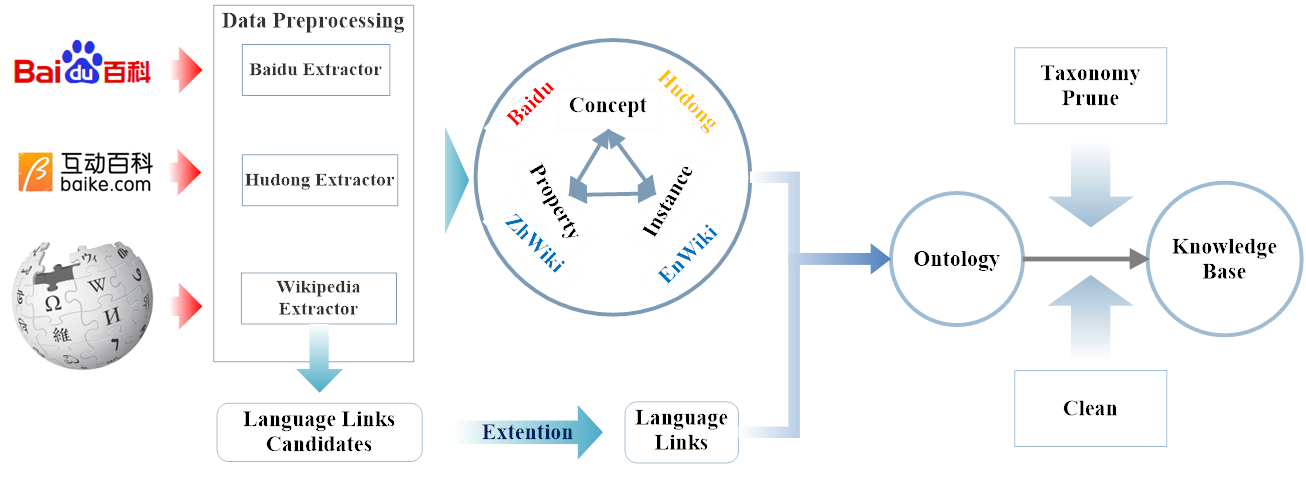
\includegraphics[width=1\columnwidth]{fig/procedure}}
    \label{fig:procedure}
    \caption{Procedure of building our cross-lingual knowledge base}
\end{figure}%
We extract information from four source, Baidu Baike, Hudong Baike, Chinese Wikipedia and English Wikipedia. Because the different data format of each source, that is, html code page of Baidu and Hudong with different layout, and XML format of Wikipedia dump file, various extractors should be applied. After file parsing, we receive four datasets with concept lists, instance lists, property lists and their relations of each source. Meanwhile, an initial Chinese-English lan-link set is generated, which is then employed a link-discovery method to become a larger set. Using the extended language links, we combine the four datasets into one. At last, going through the step of taxonomy pruning and data-cleaning, we get a final knowledge base which higher accuracy.

\section{Data Preprocessing}
\label{sec:dp}
We prepare data for the knowledge base by a series of preprocessing operations. During this stage, our goal is to get a structured dataset includes concepts, which are extracted from category taxonomy; instances, which are defined according to articles and properties, which are based on infobox and also templates assistant. We will describe the extraction approach in detail.

\subsection{Concept Extraction}
\label{sec:ce}
A concept is defined as a type of similar instances. For example, the concept of instance \emph{Interstellar} is \emph{Movie}. In general, a concept has super classes and sub classes, which means it has \emph{subClassOf} relation with other classes. Concepts comprise a taxonomy which presents a backbone of an ontology.

In an encyclopedia, a category groups several articles and also has super-categories and sub-categories, just like concept does. Therefore we can extract concepts based on existing category system. 

However, the whole taxonomy can not directly transform from category system because of the following problems:
\begin{itemize}
    \item There are auxiliary categories in Wikipedia, which help arrange specific articles or category pages. For example, \emph{Lists of artists} or \emph{Food templates}.
    \item Some sub-category links in the category system maybe inconsistent. Some categories may contain itself as sub-category, or contain sub-category that also be the super-category of it. As Fig. \ref{fig:category-mistakes} shows: In Hudong, the sub-category of 国家元首(Head of State) contains itself as a child, which causes a circle in taxonomy tree. Meanwhile, in Wikipedia, \textcolor{red}{例子}
    \item Some categories relate to only one or two articles. According to the definition of concept, such categories are less representive to a group of instances, therefore it's unwise to retain it as concept.
\end{itemize}
   To receive a cleaner and preciser concept taxonomy, we firstly do some refining works as follow:
\begin{itemize}
    \item Delete list categories or template categories in Wikipedia.
    \item Delete inconsistent sub-categories and keep the super one.
    \item Delete categories that relate to less than two articles.
\end{itemize}
The cleaning works are carried out in all encyclopedias are consistency when extracting. The remaining categories comprise an original concept taxonomy. A category and its sub-categories are correlated by the relation \emph{SubClassOf}, and a category and its articles are correlated by the relation \emph{InstanceOf}. However, there are still incorrect samples in the two relations. For example, \emph{Tsinghua University} is not an entity of \emph{Haidian District}, but relates to. Thus we will prune the taxonomy later.

\subsection{Property Extraction}
\label{sec:pe}
A property is defined as an attribute of entity. It represents the relation between two instances or an instance and its value. We divided properties into two types: object property, whose value is an individual, such as \emph{directed by}; datatype property, whose value is a text literal, such as \emph{birth date}. Considering both content and infobox of an article, we extract two groups of properties, general-properties and Infobox-properties.

\subsubsection{General-properties}
Characteristics of an entity are seen as general-properties, including label, abstract, and url. Those properties describe specific information of an entity. The label property identifies a unique entity, whose value is article title. The abstract property provides a brief description of an entity, whose value is the first paragraph of article. The url property saves the resource of an entity, which is actually a url in each source. All of them are datetype properies.

\subsubsection{Infobox-properties}
Attributes acquired from infobox are considered as Infobox-properties, such as 上映时间(release date), 导演(directed by) in a movie's infobox. All attributes relate with a typical value in the infobox. The value maybe a text or a reference to anothor entity. The type of a property, datatype or object, depends on the value. Ordinarily, a plain text value marks the property as datetype while an entity reference determines the property as object. For example, the attribute 上映时间(release date) can be defined as a datatype property as its value is a datetime string. Meanwhile, 导演(directed by) can be an object property because its value points to a person who directed the movie.

We occur some chanllenges when extracting properties from infoboxes:
\begin{itemize}
    \item The attribute label displayed in webpage infobox is inconsistent with it in dump file of Wikipedia. Fig.\ref{fig:infobox-template} gives a mapping result of display label and dump label in \emph{Interstellar}' infobox. The left is infobox while the other is a snap from dump file in Wikipedia. This movie's infobox follows template \emph{Infobox film}, where dump labels come from. Obviously the two labels are similar but not the same. As the property labels from Hudong Baike and Baidu Baike are equal to text displayed on the webpage, we have to explore the display labels in Wikipedia rather than dump labels extracted from data file.
    \begin{figure}[ht]
        \centerline{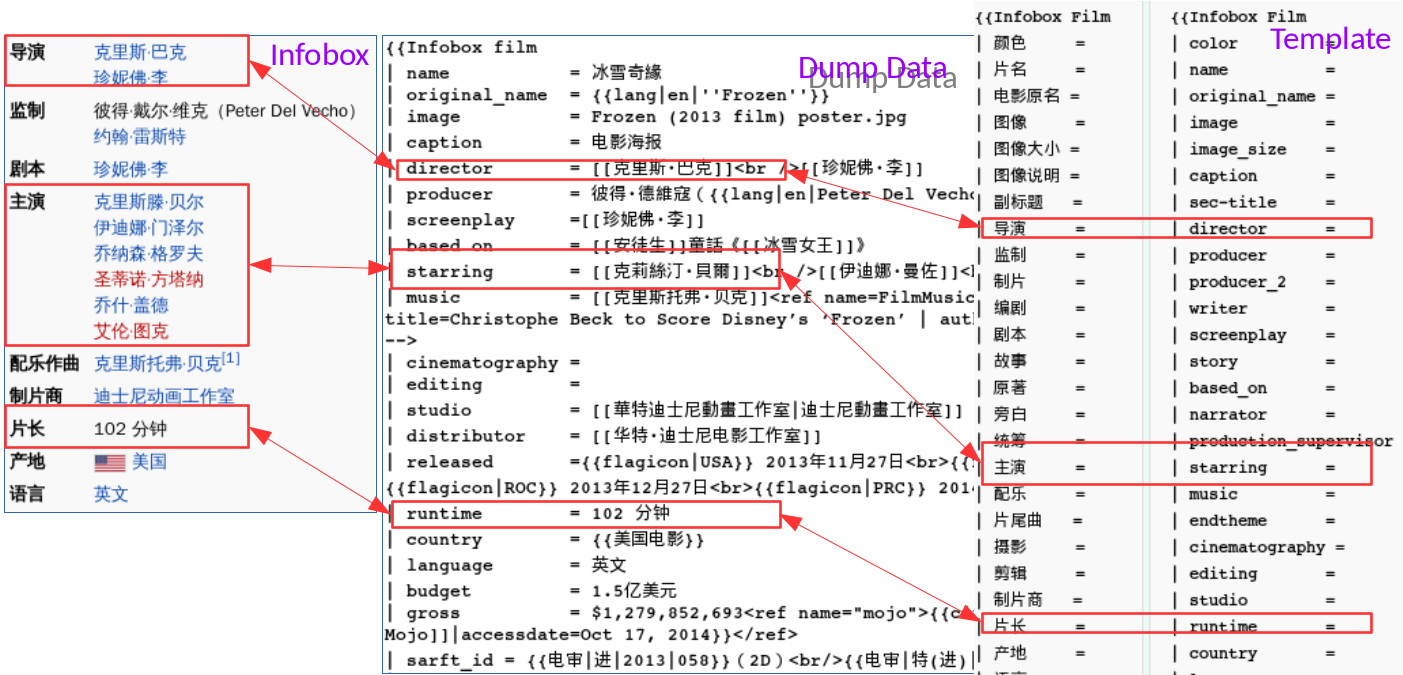
\includegraphics[width=1\columnwidth]{fig/infobox-template}}
        \label{fig:infobox-template}
        \caption{Comparison of display label and dump label in \emph{Interstellar} infobox}
    \end{figure}%
    \item There are special characters in labels. For example, Wikipedia usually use hyphen "-" or dot "•" to mark sublabels. Population property have sub-properties of "Density" and "Urban". In addition, odd signs, such as colon or asterisk, may occur in Baidu or Hudong property labels by mistake.
\end{itemize}

To solve the problems above, we take advantage of template information. Specifically, Wikipedia institutes rules of rendering label in templates. Fig.\ref{fig:infobox-render-rule} shows part of rules in \emph{template:infobox film}. When a dump label in triple-bracket occurs in a dump page, we can replace it by its mapping display label. After collecting all the display labels, we make a filter to redress the label text.

\subsection{Instance Extraction}
\label{sec:ie}
In encyclopedia, an article describes an unique entity in the world. Therefore we can extract article content as an instance. But we can't transform all the articles as instances because there are many illustrative or structure-related articles in Wikipedia, including category List pages and template documentations.

Each instance contains relations with concepts and properties. Take the movie 星际穿越(Interstellar) in Fig.\ref{fig:interstellar} as an example, concepts are assigned according to the category tags below the article page. 美国科幻片(American science fiction films) is a concept to Interstellar. In the meantime, we obtain label property from article title, which is 星际穿越(Interstellar) and abstract property from the first paragraph. Infobox-properties are also acquired via extracting from infobox in the article. Besides, according to links placing in content, we gain the reference between the current instance to others, such as 华纳兄弟(Warner Bros.).

After the preprocessing above, we harvest two types of information. One is the characteristics of instance, including instance-label, instance-abstract. The other is relationships, containing concept-instance, instance-property-value and instance-instance.

\section{Cross-lingual Knowledge Base Building}
\label{sec:clkbb}
To construct a cross-lingual knowledge base with existing structured data, firstly we gathor cross-lingual links which can help match the same entity in two languages and extend the link set. Secondly, we link the four encyclopedia, which is to say, combining concept, instance and property of the four sources into one if it represents the same thing. Thirdly, we prune the taxonomy which generates from concept relationships to retain a more accurate one. At last, we hung instances and properties on to taxonomy to create a complete knowledge base.

\subsection{Cross-lingual Links}
Wikipedia has \textcolor{red}{number} cross-lingual links between English and Chinese. By extracting language links from Wikipedia, we can get an initial cross-lingual link set of concepts and instances. Moreover, we utilize the language-independent method in \cite{wang2012cross} to extend the language-link set. With the linkage factor graph model, we harvest a cross-lingual links extension as many as 20 thousands with an ideal precision 85.5\% and a recall of 88.1\%.

However, due to following templates, Infobox-properties have no obvious cross-lingual links. To aquire such links, we go through the following steps: (1) Given a matched template, that is a template has infobox rules in both English and Chinese, find the mapping pairs; (2) Given the English and Chinese infoboxes of a matched instance, compare the templates they use, find the matched label mapping to the same dump label. (3) Given the English and Chinese infoboxes of a matched instance, to datatype properties, compare the similarity of literal value; to object properties, check whether the value refer to the same entity. The whole process can be summarized as Algorithm \ref{alg:ple}. Some of the symbols have already denoted in \ref{sed:definition}
\subsection{Cross-lingual Linking}
In order to make the ontology of one encyclopedia link to others, we unify the same concept, instance and property from four source to unique one and make identifier. For example, we merge instances by the following method:

\begin{enumerate}[1)]
    \item Given an instance extracted from Chinese Wikipedia, find the entity in Hudong and Baidu Baike with the same title. 
    \item Given an instance extracted from Hudong, find the entity which is not in Chinese Wikipedia but in BaiduBaike with the same title.
    \item The other instances existing in only one encyclopedia are considered as an independent instance. Up to now, we have combined all Chinese articles describing the same entity as one instance. Each instance may correspond to 1 to 3 sources.
    \item To a $L_{z}(a)$, which is same as $Ti(a)$, find whether there is an English cross-lingual link in $CL<L_{e}, L_{z}>$. If exists, make the two as one instance and identify it using an ID.
    \item If a $L_{z}$ or a $L_{e}$ has no matched cross-lingual link, number it with an independent ID.
\end{enumerate}

After the above steps, we acquire a list of instances and their unique IDs. Some of them contain cross-lingual information while some contain monolingual.

The process of unify concept and property is the same as instance. Meanwhile, all the relations in all sources are kept to prevent loss of information. 

\subsection{Taxonomy Prune}
\label{sec:tp}
As a result of combining multi source information without verifying, the taxonomy of concept system is mussy. For example, \textcolor{red}{example}. Therefore, we introduce the method from\cite{wang2014cross} to filter the correct subClassOf and instanceOf relations between two entities. Table. \ref{tab:} shows some examples of correct relations. In particular, some language-dependent literal and language-independent structural features are defined to vector each concept or instance. The literal features include the head words’ singular/plural forms of labels of English entities, the prefix/suffix relation of labels of Chinese entities. The structural features include article divergence for subClassOf, property divergence for subClassOf, category divergence for subClassOf, article divergence for instanceOf, property divergence for instanceOf, category divergence for instanceOf. By employing these features, a binary-classification model is trained based on Logistic Regression. The whole process is iterative by add assured result into training set and retraining the model to get higher precision. Confirming a right subClassOf or instanceOf not only depends on the prediction result of classification, but also related with cross-lingual knowledge validation, which ensures correctness if both the mapped English and Chinese relations are right. Fig. \ref{fig:} shows an example of the process.

The ideal result of pruning is a tree, whose lines denote relations, nodes denote concepts and leaves denote instances. However, with wrong relations cut without caring about integrity, getting a forest is inevitable. We may lose some links but get more accurate relations instead.

\subsection{Knowledge Base Building}
To build a knowledge base, we first define specific URI to identify each element in the prepared dataset. URIs of concept, instance, and property are created by concatenating a namespace prefix and ID. Table \ref{tab:uris} lists the URI defined in the knowledge base.
\begin{table}[h]
\small
\centering
\caption{URIs for concept, instance, property in our knowledge base}
\label{tab:uris}
    \begin{tabular}{|c|c|}
        \hline
        Type     & URI                          \\ \hline
        Concept  & http://xlore.org/concept/id  \\ \hline
        Instance & http://xlore.org/instance/id \\ \hline
        Property & http://xlore.org/property/id \\ \hline
    \end{tabular}
\end{table}

\section{Result}
\label{sec:result}
\subsection{DataSet}
四个百科的数据统计,包括我们有的百科数据的发布时间,格式(xml。html),article数量,抽取的instance数量,concept数量,property数量, wiki中跨语言链接数量
其实最好有一些我们在抽取过程中删剪的不符合要求的concept或者property数量,不过要看有没有时间再跑一下了
\subsection{Extracted Knowledge Base}
xlore 的统计数据,包括instance数量,concept数量,property数量,有双语的instance、concept、property,只有中文的,只有英文的
顶层分类以及下属concept和instance数量
有最多instance的property(object property),以及相应的instance数量
有最多的text的property(datatype property),以及数量
删除的taxonomy关系(如果重做实验的话)

\subsection{Query Interface}
各种我们自己定义的uri,比如abstract,reference。。。。
各种查询语句示例

\section{Related Work}
\label{sec:work}
In this section, we introduce some related knowledge bases and cross-lingual knowledge linking methods are referred to.
\subsection{Chinese Knowledge Bases}
Currently, several large-scale Chinese knowledge bases have been generated. Zhishi.me\cite{niu2011zhishi,wang2014publishing} is the first large-scale Linking Open Data published. It acquires structural information from three original sources, Chinese Wikipedia, BaiduBaike and Hudong and gets more than 5 million distinct entities. Zhishi.me helps generate knowledge base focused on relations in Junfeng Pan’s work\cite{pan2012building}. 
Similar with Zhishi.me, CKB\cite{wang2012building} is created from Hudong Baike. It first learns an ontology based on category system and properties, and then collects 19542 concepts, 2381 properties, 802593 instances. Besides using existing encyclopedias, CASIA-KB employs other types of sources(e.g. microblog posts, news pages, images) to enrich the structured knowledge.
\subsection{Cross-lingual Knowledge Bases}
DBpedia \cite{auer2007dbpedia,mendes2012dbpedia} is one of the most used cross-lingual knowledge base in the world. It's extracts various kinds of structured information from Wikipedia and employ the multilingual characteristic of Wikipedia to generate 97 language versions of content. This knowledge base is widely applied in many domain, including media recommendation \cite{passant2010dbrec,fernandez2011generic,kaminskas2012knowledge}, entity linking\cite{mendes2011evaluating} and information extraction \cite{dutta2013integrating}.
Universal WordNet(UWN)\cite{de2012uwn} is a large multilingual lexical knowledge base which is build from WordNet and enriched its entities from Wikipedia. It is constructed using sophisticated knowledge extraction, link prediction, information integration, and taxonomy induction methods. The API is available to over 200 languages and more than 16 million words and names. UWN provides semantic relationship of list of word meanings for Aya's work on conceptual search \cite{al2015conceptual} 

\subsection{Cross-lingual Knowledge Linking}
Discovering more cross-lingual links is benefit to development of a multilingual knowledge base. General method is divided into two steps. First find missing link candidates using link structure of articles and then decide whether candidates are cross links or not by classification. \cite{sorg2008enriching} employs such approach to resolve the problem of automatically inducing new cross-language links. Wang\cite{wang2012cross} utilize a linkage factor graph model 

\section{Conclusion}
\label{sec:con}

%\section*{Acknowledgement}
%Thanks anonymous reviewers for their valuable suggestions that help us improve the quality of the paper. Thanks Prof. Chua Tat-Seng from National University of Singapore for discussion. The work is supported by 973 Program (No. 2014CB340504 ), NSFC-ANR (No. 61261130588), Tsinghua University Initiative Scientific Research Program (No. 20131089256) and THU-NUS NExT Co-Lab.

\bibliographystyle{splncs03}
\bibliography{paper}

\begin{algorithm}[t]
    \KwIn{ English Infobox template set $TS_{e}$, Chinese Infobox template set $TS_{z}$, English article set $AS_{e}$, Chinese article set $AS_{z}$, existing lan-link map $CL<L_{e}, L_{z}>$ }
\KwOut{Property lan-link map $CL_{p}$}

Initialization: $CL_{p} = \{\} $\\
\ForEach {English Template $T_{e} \in TS_{e}$}{
    $L_{e}$ = label of $T{e}$ \\
    \eIf {$L_{e} \in CL$}{
        $L_{z} = CL\left[L_{e}\right] $ ,\ $T_{z} = TS_{z}\left[L_{z}\right]$\\
        \ForEach{$tl \in T_{e}.pset.tlset \cap T_{z}.pset.tlset $}{
            $CL_{p}$.add(<$T_{e}.p[tl].dl$, $T_{z}.p[tl].dl$>)
        }
    }
}

\ForEach {English Article $A_{e}$ \in $AS_{e}$}{
    $L_{e}$ = label of $A_{e}$ 
    \eIf {$L_{e} \in CL$}{
        $L_{z} = CL\left[L_{e}\right]$ ,\ $A_{z} = AS_{z}\left[L_{z}\right]$ \\

        $T_{e}$ = Template of $A_{e}$.I ,\ $T_{z}$ = Template of $A_{z}$.I \\

        Set $Cset$ as the Common set of template labels of $T_{e}$ and template labels of $T_{z}$ \\
        $Cset = T_{e}.pset.tlset \cap T_{z}.pset.tlset $ \\

        \ForEach {template label $tl \in Cset $}{
            $CL_{p}$.add(<$T_{e}.pset[tl].dl$, $T_{z}.pset[tl].dl$>)
        }

        \ForEach{English template label $tl_{e} \in T_{e}.pset.tlset \minus Cset$}{
            $p_{e} = T_{e}.pset\left[tl_{e}\right]$ \\
            \ForEach{Chinese template label $tl_{z} \in T_{z}.pset.tlset - Cset$}{
                $p_{z} = T_{z}.pset\left[tl_{z}\right]$ \\
                \eIf {$p_{e}.type$ is datatype $\&\&$ $p_{z}.type$ is datatype}{
                    \eIf {CalculateSimilar($p_{e}.v$, $p_{z}.v$) > $threshold$}{
                        $CL_{p}$.add(<$p_{e}.dl$, $p_{z}.dl$>)
                    }
                } \eElseIf {$p_{e}.type$ is object $\&\&$ $p_{z}.type$ is object}{
                    \eIf{ReferToCommmonEntity($p_{e}.v$, $p_{z}.v$)}{
                        $CL_{p}$.add(<$p_{e}.dl$, $p_{z}.dl$>)
                    }
                }
            }
        }
    }
}
\caption{Property Links Extraction}
\label{alg:ple}
\end{algorithm}

\end{document}

